

\section{Zielsetzung}
 Mithilfe der Faraday-Rotation, eine magneto-optische Untersuchung, können Informationen über die Banstrukturen von Halbleitern
 gewonnen werden. Ziel dieses Versuchs ist es, die effektive Masse von Elektronen des Halbleiters Galliumarsenid zu bestimmen.
\section{Theorie}
\subsection{Effektive Masse}
Für die Beschreibung der Bandstrukturen von Halbleitern ist es häufig ausreichend
die Form der unterste Bandkante des Leitungsbandes zu untersuchen. Dies ist in Abbildung \ref{fig:bandstruktur} zu sehen.
Dort wird die Elektronenenergie $\su{\varepsilon}$ in Abhängigkeit der Wellenzahlvektoren $\su{\vec{k}}$ dargestellt.
\begin{figure}
    \centering
    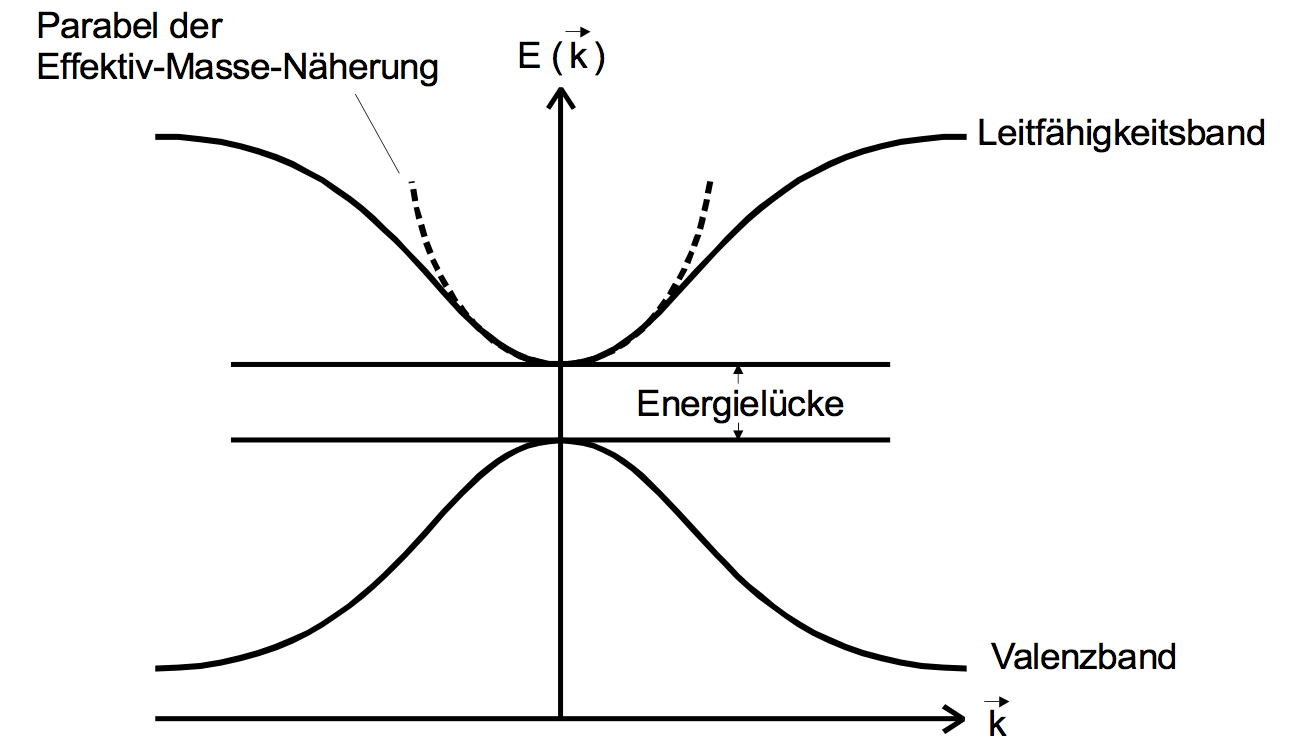
\includegraphics[scale = 0.4]{bandstruktur.png}
    \caption{Vereinfachte Darstellung einer Energiebandstruktur eines Festkörpers.\cite{1}}
    \label{fig:bandstruktur}
  \end{figure}
 \newline
Zur Vereinfachung der Funktion $\varepsilon(\vec{k})$, welche die Form der Energiebänder beschreibt, wird diese in eine Taylorreihe entwickelt
und davon ausgegangen, dass die untere Bandkante im Koordinatenursprung liegt. Daraus folgt
\begin{equation}
 \varepsilon(\vec{k}) = \varepsilon(0) + \frac{1}{2} \sum_{i=1}^3
  \bigg(\frac{\partial \epsilon^2}{\partial k_i^2}\bigg)_{k=0} k_i^2 + ...\
\end{equation}
Durch den Vergleich mit
\begin{equation*}
  \varepsilon = \frac{\hbar^2 k^2}{2 m}
\end{equation*}
wird deutllich, dass die effektive Masse, welche durch
\begin{equation*}
  m_i^* \coloneqq \frac{\hbar^2}{\Big\{\frac{\partial^2\epsilon}{\partial k_i^2}\Big\}_{k=0}}
\end{equation*}
beschrieben wird, die Dimension einer Masse haben muss. Für einige Kristalle ist die Symmetrie so hoch, dass die $m_i^*$ gleich sind und diese deswegen als $m^*$ geschrieben
werden können. \newline
Dies ermöglicht, dass die Elektronen in den Bändern wie freie Elektronen behandelt werden können. In der Schrödinger-Gleichung wird dann
die Masse durch die effektive Masse ersetzt und die Quantenmechanik freier Teilchen ist für die eigentlich
gebundenen Elektronen gültig.

\subsection{Zirkuläre Doppelbrechung bei optisch aktiver Materie}
\begin{figure}
    \centering
    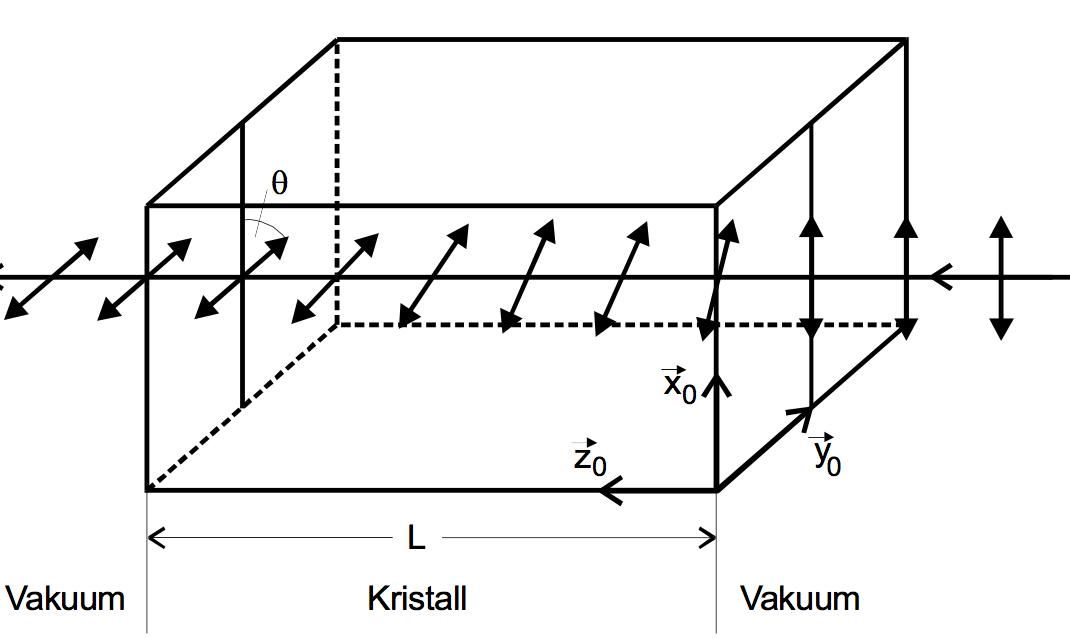
\includegraphics[scale = 0.4]{polarisationsache.png}
    \caption{Drehung der Polarisationsebene beim Durchgang durch einen Kristall .\cite{1}}
    \label{fig:polarisationsache}
  \end{figure}
 Bei der zirkulären Doppelbrechung kommt es beim Durchgang eines Lichtstrahls durch einen Kristall
 zur Drehung der Polarisationsebene, wie in Abbildung \ref{fig:polarisationsache} zu sehen ist. Dies geschieht allerdings nur bei optisch aktiver Materie.
 Zur Erklärung der zirkulären Doppelbrechung wird davon ausgegangen, dass es sich bei dem linear-polarisierten Licht um eine Überlagerung
 eines rechts- und linkszirkulären Teilstrahls, die sich mit unterschiedlichen Phasengeschwindkeiten $v_{\su{ph}}$ und Wellenzahlen $\su{k}$ ausbreiten, handelt. Dadurch erfährt der zuvor linear-polarisierte Stahl seine Drehung.
 Der Rotationswinkel wird durch
\begin{align*}
    \theta &=\frac{L}{2} \left(k_{\text{R}}-k_{\text{L}}\right)\\
          &=\frac{L\omega}{2}\left(\frac{1}{v_{\text{ph}_{\text{R}}}}-\frac{1}{v_{\text{ph}_{\text{L}}}}\right)\\
\end{align*}
berechnet. Dabei ist L die Kristalllänge und $\omega$ die Frequenz des einfallenden Strahls. \newline
Die zirkuläre Doppelbrechung entsteht durch induzierte Dipolmoment, da permanente Dipole aufgrund ihrer
längeren Relaxationszeit der Frequenz des Lichtes nicht folgen können. \newline
Die Dipole erzeugen eine Polarisation des Kristalls der Form
\begin{equation*}
    \vec{P} = \epsilon_0 \chi \vec{E}.
\end{equation*}
Diese ist abhängig von dem elektrischen Feld und der dielektrischen Suszeptibilität $\chi$, die für anistrophe
Kristalle als Tensor definiert ist. Durch den nicht-diagonalen Tensor und den komplex konjuierten Koeffizienten
wird die Materie doppelbrechend.\newline
Der Tensor sieht dann wie folgt aus
\begin{equation*}
    ( \chi ) =
    \begin{pmatrix}
      \chi_{\text{xx}} & i\chi_{\text{xy}} & 0 \\
      -i \chi_{\text{xy}}& \chi_{\text{xx}} & 0 \\
      0& 0 & \chi_{\text{zz}}
      \end{pmatrix}.
\end{equation*}
Der Rotationswinkel wird durch
\begin{equation}
  \theta = \frac{L \omega}{2 c n} \chi_{xy}.
  \label{eqn:1}
\end{equation}

genähert.

\subsection{Zirkuläre Doppelbrechung bei optisch inaktiver Materie}
Wie bereits erwähnt, kommt es bei optisch aktiver Materie zur zirkulären Doppelbrechung.
Bei optisch inaktiver Materie hingegen kann es zur zirkulären Doppelbrechung nur durch das Anlegen eines Magnetfeldes
kommen. Dies wird als Faraday-Effekt bezeichnet. \newline
Durch die Vernachlässigung der Dämpfungseffekte und des Einflusses des Magnetfelds der elektromagnetischen Lichtwelle
wird die Verschiebungspolarisation durch
\begin{equation*}
    \vec{P} = -Ne_0\vec{r}
\end{equation*}
beschrieben, wobei $\vec{r}$ die Auslenkung der Elektronen aus der Gleichgewichtslage beschreibt.
Damit kann das Tensorelement $\chi_{\text{xy}}$ für Gleichung \ref{eqn:1} bestimmt werden.
\newline
Mit der Bewegungsgleichung für ein gebundenes Elektron mit der Masse m und Ladung $\su{e_0}$
\begin{equation*}
    m\frac{d^2\vec{r}}{dt^2} + K\vec{r} = -e_0\vec{E}(r) -e_0\frac{d\vec{r}}{dt}\times\vec{B}
\end{equation*}
kann der Rotationswinkel wie folgt bestimmt werden
\begin{equation*}
  \theta(\lambda)=\frac{2\pi^2 \text{e}_0^3 \text{c}}{\epsilon_0}\frac{1}{{m^*}^2
  \lambda^2 \omega{_0}^4}\frac{N B L}{n}
\end{equation*}
und ist damit proportional zur Flussdichte B, der Probenlänge L und der Anzahl der Ladungsträger N
pro Volumeneinheit. Für den Fall $\omega_0 \rightarrow 0$ der Resonanzfrequenz folgt für die nahezu freien Ladungsträger
ein Drehwinkel der Polarisationseben von
\begin{equation}
  \theta_{\text{frei}}(\lambda)=\frac{\text{e}_0^3}{8 \pi^2 \epsilon_0 \text{c}^3}
  \frac{\lambda^2}{{m^*}^2}\frac{N L B}{n}.
  \label{eqn:meff}
\end{equation}
Dieser Zusammenhang ist durch das Ersetzen der Masse auch für Kristallelektronen gültig und wird deswegen zur Bestimmung der
effektiven Masse verwendet.

\newpage
\section{Versuchsaufbau}
Der Versuchsaufbau ist in Abbildung \ref{fig:aufbau} dargestellt.
\begin{figure}
    \centering
    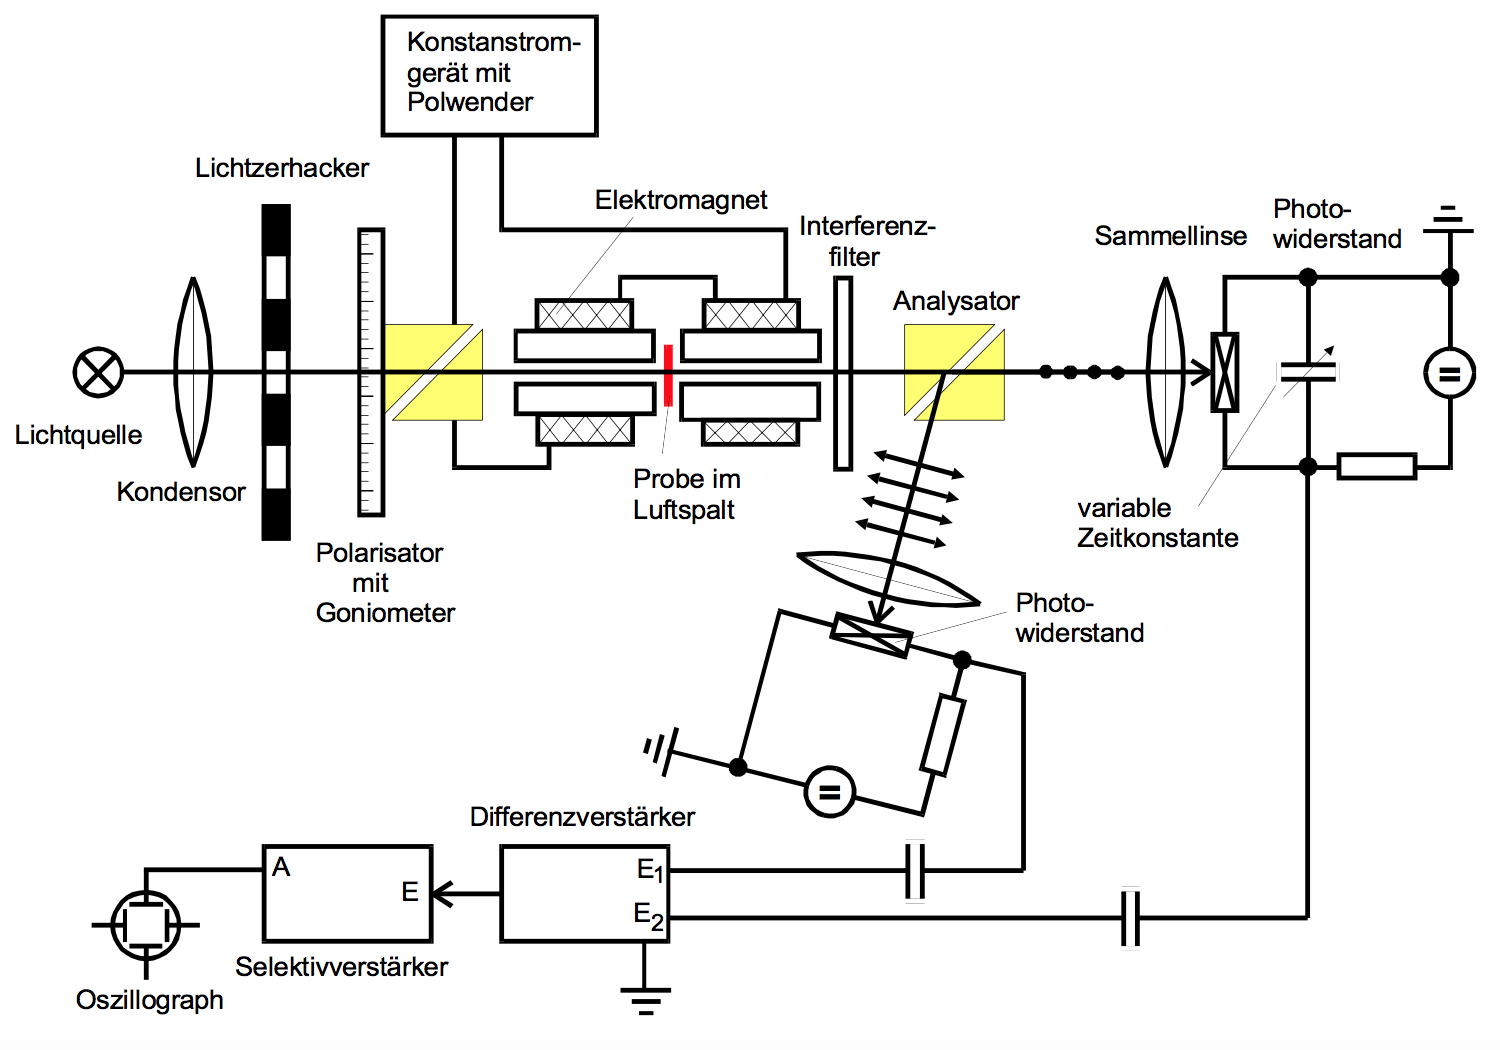
\includegraphics[scale = 0.4]{aufbau.png}
    \caption{Versuchsaufbau.\cite{1}}
    \label{fig:aufbau}
  \end{figure}
 \newline
Das emittierte Infrarotlicht einer Halogen-Lampe wird von einer Kondensorlinse gebündelt,
durch einen Interferenzfilter, welche aus einer Strahlung einen kleinen Wellenlängenbereich herausfiltert,
monochromatisiert und durch ein Glan-Thompson-Prisma aus Kalkspat linear polarisiert.
Die scheibenförmige Probe wird in einen Elektromagneten eingeführt, welcher an ein Konstantstromgerät
angeschlossen ist. Ein weiteres Glan-Thompson-Prisma hinter dem Elektromagneten spaltet den Lichtstrahl
in zwei senkrecht zueinander polarisierte Teilstrahlen auf. Durch einen Lichtzerhacker, welcher den Photowiderständen
vorgelagert ist, fällt eine Wechselspannung statt einer Gleichspannung an den Photowiderständen ab.
Mit diesen kann die Intensität beider Strahlen bestimmt werden.
Die Differenz der abfallenden Signalspannungen werden dann über einen Differenzverstärker und einem
Selektivverstärker auf einem Oszilloskop sichtbar gemacht. Dies führt dazu, dass die Störspannungen
weitgehend unterdrückt werden. Der Selektivverstärker ist dabei auf die Zerhackerfrequenz abgestimmt.
\section{Versuchsdurchführung}
Zur Justierung der Apparatur mit sichtbaren Licht wird zunächst der Interferenzfilter
entfernt. \newline
Als erstes wird die Genauigkeit der Polarisationsvorrichtung überprüft. Dafür wird das zweite Glan-Thompson-Prisma
um seine vertikale Achse so gedreht, dass keine Lichtintenstiät für den durchgehenden Strahl des ersten Glan-Thompson-Prismas
messbar ist. \newline
Durch die Einstellung des Abstandes zwischen der Sammellinse und den Photowiderständen wird die Abbildung der Lichtquelle
auf die lichtempfindlichen Flächen der Widerstände überprüft.\newline
Als nächstes wird die Zerhackerfrequenz eingestellt und die Frequenz des Selektivverstärkers an diese
angepasst. Mithilfe eines Oszilloskops kann dieses Verhältnis dargestellt werden. Zur Unterdrückung der
Störspannungen wird die Ausgangsspannung des Selektivverstärkers auf seinen maximalen Wert eingestellt.\newline
Auch die Lichtintentsität wird eingestellt. Hierbei wird durch die relative Verschiebung der Lichtquelle und der
Sammellinse zum Lichtzerhacker versucht, die Intensität noch zu erhöhen.\newline
Dann erst wird der Interferenzfilter und die zu untersuchenden Probe in die Apparatur hinzugefügt.
Vor der Messung der Winkel wird erneut das Signal abgeglichen.

Zur Bestimmung des Rotationswinkels $\su{\theta}$ wird die Lichtintensität der Teilstrahlen auf den gleichen
Wert eingestellt, damit keine Spannung am Ausgang des Differenzverstärkers mehr messbar ist.
Am Polarisator kann mittels eines Goniometers der durch das Magnetfeld entstandene Winkel abgelesen werden.
Danach wird das Magnetfeld umgepolt und der Winkel erneut abgelesen. Mit der Formel
\begin{equation*}
    \theta= \frac{1}{2}(\theta_1-\theta_2)
\end{equation*}
ist der Rotationswinkel zu berechnen.\newline
Die Rotationswinkel werden für hochreines und n-dotiertes Galliumarsenid für acht Wellenlängen im nahen
Infrarotbereich gemessen.\newline
Mit einer Hallsonde wird in Richtung des einfallenden Strahles das maximale Magnetfeld ausgemessen.
